% https://mirrors.ibiblio.org/CTAN/fonts/fontawesome/doc/fontawesome.pdf
\documentclass[a4paper,12pt, final]{article}
% Adjust the page margins if needed
% \usepackage[scale=0.75]{geometric}
% \usepackage[utf8]{inputenc}
\usepackage[english]{babel}
\usepackage[
    ignoreheadfoot, % set margins without considering header and footer
    top=2cm, % separation between body and page edge from the top
    bottom=3cm, % separation between body and page edge from the bottom
    left=2cm, % separation between body and page edge from the left
    right=2cm, % separation between body and page edge from the right
    footskip=1.5cm, % separation between body and footer
]{geometry} % for adjusting page geometry

\usepackage[explicit]{titlesec} % for customizing section titles
% \usepackage{tabularx} % for making tables with fixed width columns
% \usepackage{array} % tabularx requires this
\usepackage[dvipsnames]{xcolor} % for coloring text
% \definecolor{primaryColor}{RGB}{0, 79, 144} % define primary color
\definecolor{primaryColor}{RGB}{0, 0, 0} % define primary color
\usepackage{enumitem} % for customizing lists
\usepackage{fontawesome5} % for using icons
\usepackage{amsmath} % for math
\usepackage[
    pdftitle={},
    pdfauthor={},
    colorlinks=true,
    urlcolor=primaryColor
]{hyperref} % for links, metadata and bookmarks
\usepackage[pscoord]{eso-pic} % for floating text on the page
\usepackage{calc} % for calculating lengths
\usepackage{bookmark} % for bookmarks
\usepackage{lastpage} % for getting the total number of pages
\usepackage[default, type1]{sourcesanspro} % for using source sans 3 font
\usepackage{ifthen}
\usepackage{fancyhdr}
\usepackage{graphicx}
\usepackage{blindtext}

% Team Information
\newcommand{\ourteam}{}

\title{Optimizing Truck Routing and Delivery Efficiency}
% % % Header and Footer Styling
% Some settings:
\pagestyle{empty} % no header or footer
\pagestyle{fancy}
\fancyhf{} % sets both header and footer to nothing
\renewcommand{\headrulewidth}{0pt}
\fancyfoot[CO,RE]{\color{gray}\textit{\small \ourteam \ - Page \thepage{} of \pageref*{LastPage}}}



% \titleformat{\section}{
%     % make the font size of the section title large and color it with the primary color
%     \Large\color{primaryColor}
% }{
% }{
% }{
%     % print bold title, give 0.15 cm space and draw a line of 0.8 pt thickness
%     % from the end of the title to the end of the body
%     \textbf{#1}\hspace{0.15cm}\titlerule[0.8pt]\hspace{-0.1cm}
% }[] % section title formatting

% \titlespacing{\section}{
%     % left space:
%     0pt
% }{
%     % top space:
%     0.3 cm
% }{
%     % bottom space:
%     0.2 cm
% } % section title spacing

% \titleformat{\subsection}{
%     % \color{primaryColor}
% }{
% }{
% }{
%     #1 \hspace{0.15cm}\hspace{-0.1cm}
% }[] % section title formatting

% \newenvironment{header}{
%     \setlength{\topsep}{0pt}\par\kern\topsep\centering\color{primaryColor}\linespread{1.5}
% }{
%     \par\kern\topsep
% } % new environment for the header

\newcommand{\placelastupdatedtext}{% \placetextbox{<horizontal pos>}{<vertical pos>}{<stuff>}
    \AddToShipoutPictureFG*{% Add <stuff> to current page foreground
        \put(
        \LenToUnit{\paperwidth-2 cm-0.2 cm+0.05cm},
        \LenToUnit{\paperheight-1.0 cm}
        ){\vtop{{\null}\makebox[0pt][c]{
                    % \small\color{gray}\textit{Last updated in February 2024}\hspace{\widthof{Last updated in February 2024}}
                    \small\color{gray}\textit{Last updated on \today}\hspace{\widthof{Last updated on \today}}
        }}}%
    }%
}%

% save the original href command in a new command:
\let\hrefWithoutArrow\href
% new command for external links:
\renewcommand{\href}[2]{\hrefWithoutArrow{#1}{\mbox{\ifthenelse{\equal{#2}{}}{ }{#2 }\raisebox{.15ex}{\footnotesize \faExternalLink*}}}}


% For TextEntrys (see https://tex.stackexchange.com/a/600/287984):
% \def\changemargin#1#2{\list{}{\rightmargin#2\leftmargin#1\topsep=0pt\itemsep=0pt\parsep=0pt\parskip=0pt\labelwidth=0pt\itemindent=0pt\labelsep=0pt}\item[]}
% \let\endchangemargin=\endlist 

% Ensure that generate pdf is machine readable/ATS parsable
\pdfgentounicode=1
% \pagestyle{customFooterStyle}



% Begin Document
\begin{document}
% \fancyfoot[R]{}
\placelastupdatedtext
\maketitle
% % Title/Header
% \vspace{0.3 cm}

\tableofcontents

\section{Executive Summary}
This idea focuses on improving the delivery process by optimizing truck routes. The company is
currently facing high delivery costs due to inefficient truck routing.
The proposed solution involves using clustering techniques (DBSCAN or K-means) and solving the
Vehicle Routing Problem (VRP) to reduce delivery time and costs.

\section{Problem Statement}
The company is currently experiencing high logistics costs due to inefficient truck routing and
suboptimal customer clustering. This leads to increased delivery time and excessive fuel
consumption.

\section{Proposed Solution}
The solution relies on using clustering algorithms to group customers based on proximity and then
optimizing truck routes using Vehicle Routing Problem (VRP) algorithms. Trucks will be assigned
based on their capacity to maximize efficiency.

\subsection{How It Works}
\begin{enumerate}
    \item Receive customer orders and validate them.
    \item Cluster customers geographically.
    \item Assign trucks based on capacity and volume of packages.
    \item Optimize truck routes using VRP solutions.
    \item Calculate the most efficient paths for each truck.
\end{enumerate}
\subsection{Benefits of Solution}
\begin{enumerate}
    \item Reduce costs by minimizing fuel consumption.
    \item Improve efficiency by reducing delivery times.
    \item Scalability: the solution can grow as the number of trucks and customers increases.
\end{enumerate}

\section{Implementation Plan}
\begin{enumerate}
    \item Pilot test the solution in a small region.
    \item Full-scale implementation across the logistics network.
    \item Provide training to staff on the new system.
\end{enumerate}




\section{Diagrams}
\subsection{Database Diagrams}
% \blindtext

\begin{figure}[h]
   \centering
   \begin{tabular}{@{}c@{\hspace{.5cm}}c@{}}
       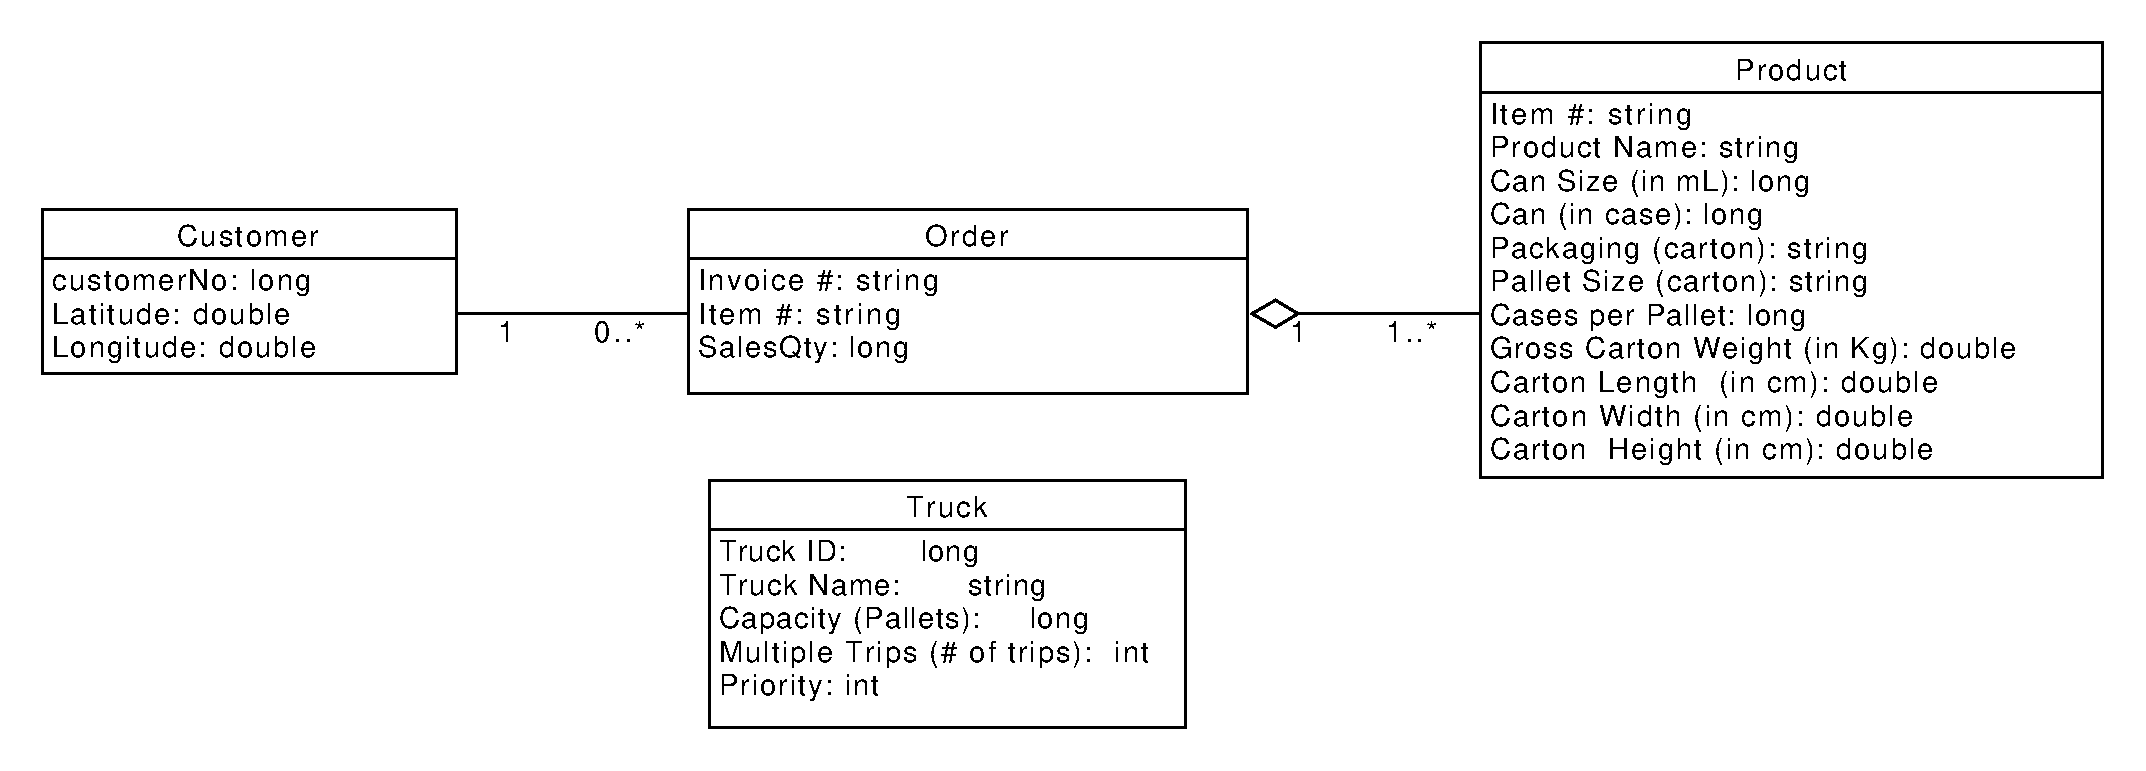
\includegraphics[page=1,width=1\textwidth]{TLDR_old_u.pdf}
       % \includegraphics[page=2,width=.45\textwidth]{somemultipagepdf} \\[.5cm]
       % \includegraphics[page=3,width=.45\textwidth]{somemultipagepdf} \\
   \end{tabular}
 \caption{Old Database Diagram}
 \label{fig:Test}
\end{figure}

% \blindtext

\begin{figure}[h]
   \centering
   \begin{tabular}{@{}c@{\hspace{.5cm}}c@{}}
       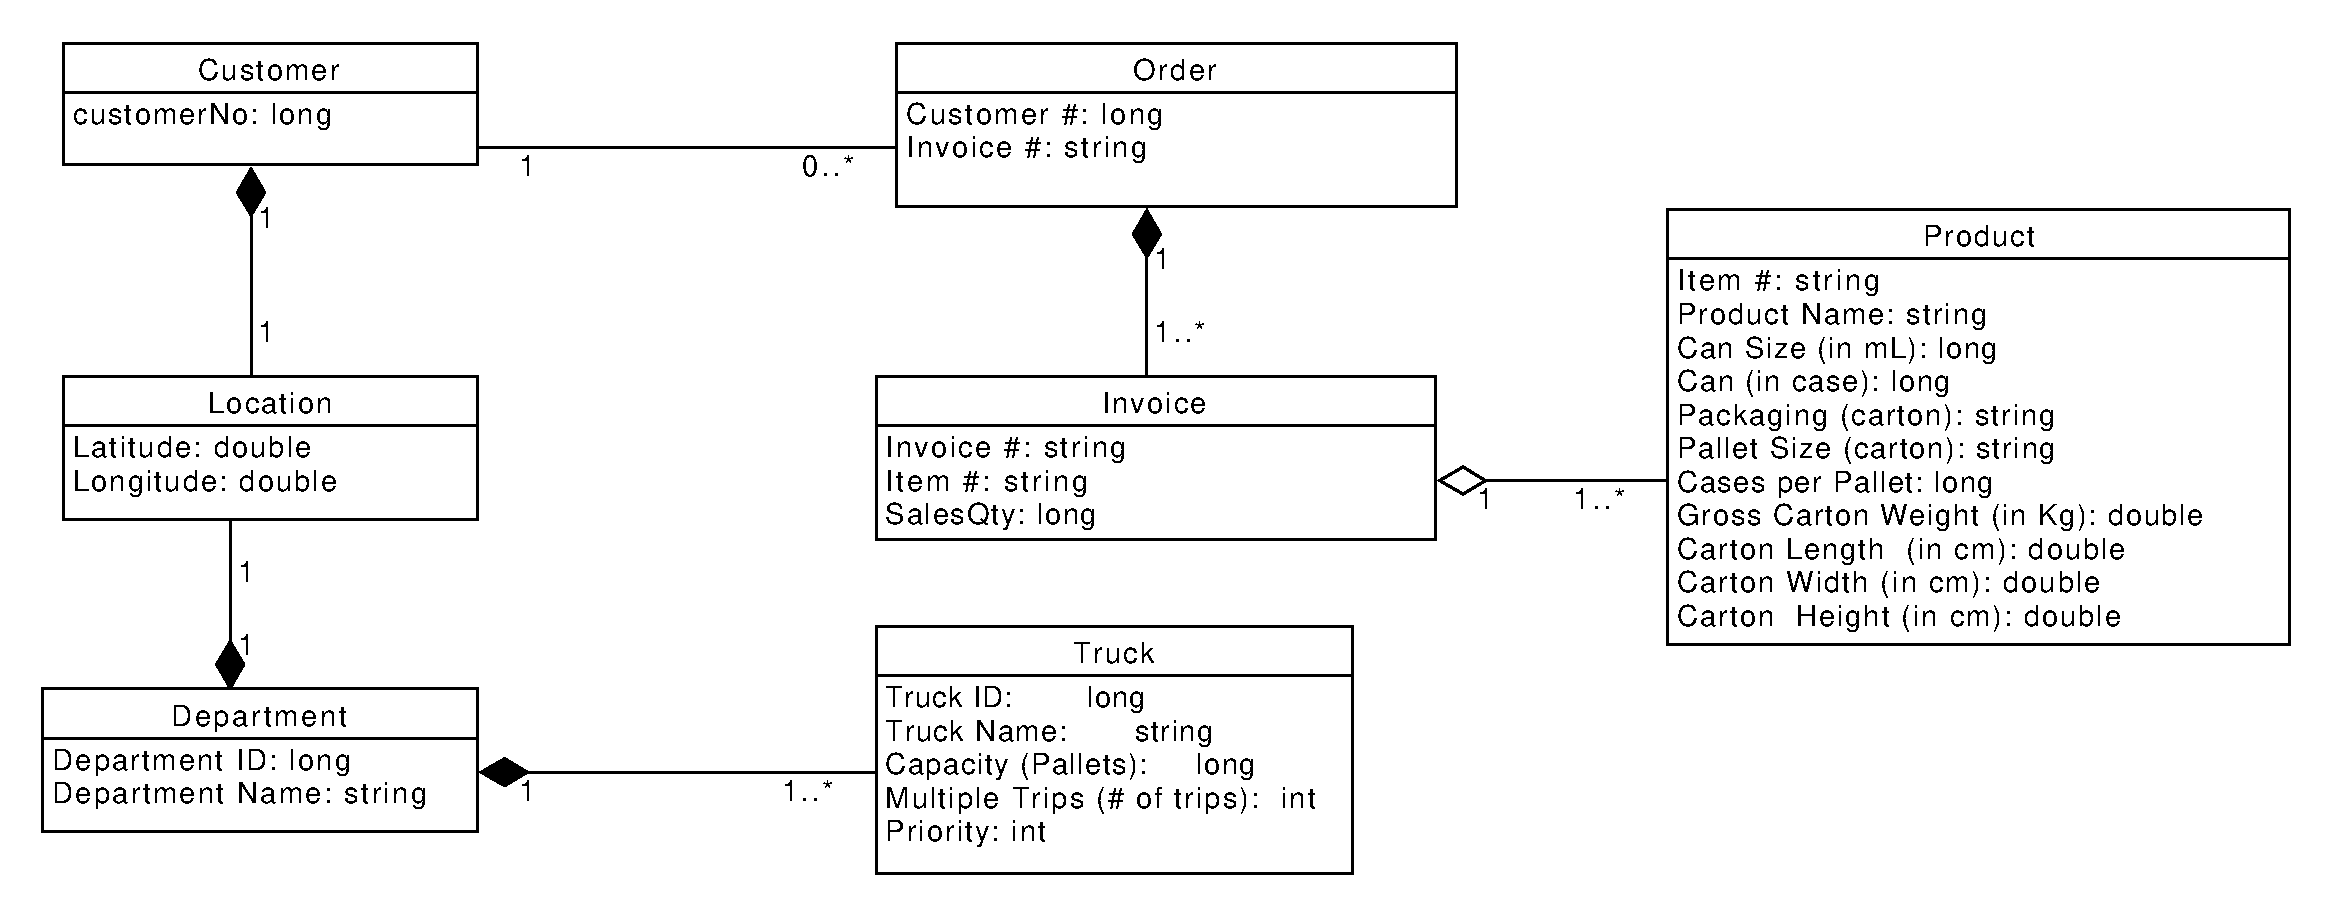
\includegraphics[page=1,width=1\textwidth]{TLDR_new_u.pdf} 
       % \includegraphics[page=2,width=.45\textwidth]{somemultipagepdf} \\[.5cm]
       % \includegraphics[page=3,width=.45\textwidth]{somemultipagepdf} \\
   \end{tabular}
 \caption{New Database Diagram}
 \label{fig:Test}
\end{figure}
\newpage
\subsection{Activity Diagrams}
\begin{figure}[h]
   \centering
   \begin{tabular}{@{}c@{\hspace{.5cm}}c@{}}
       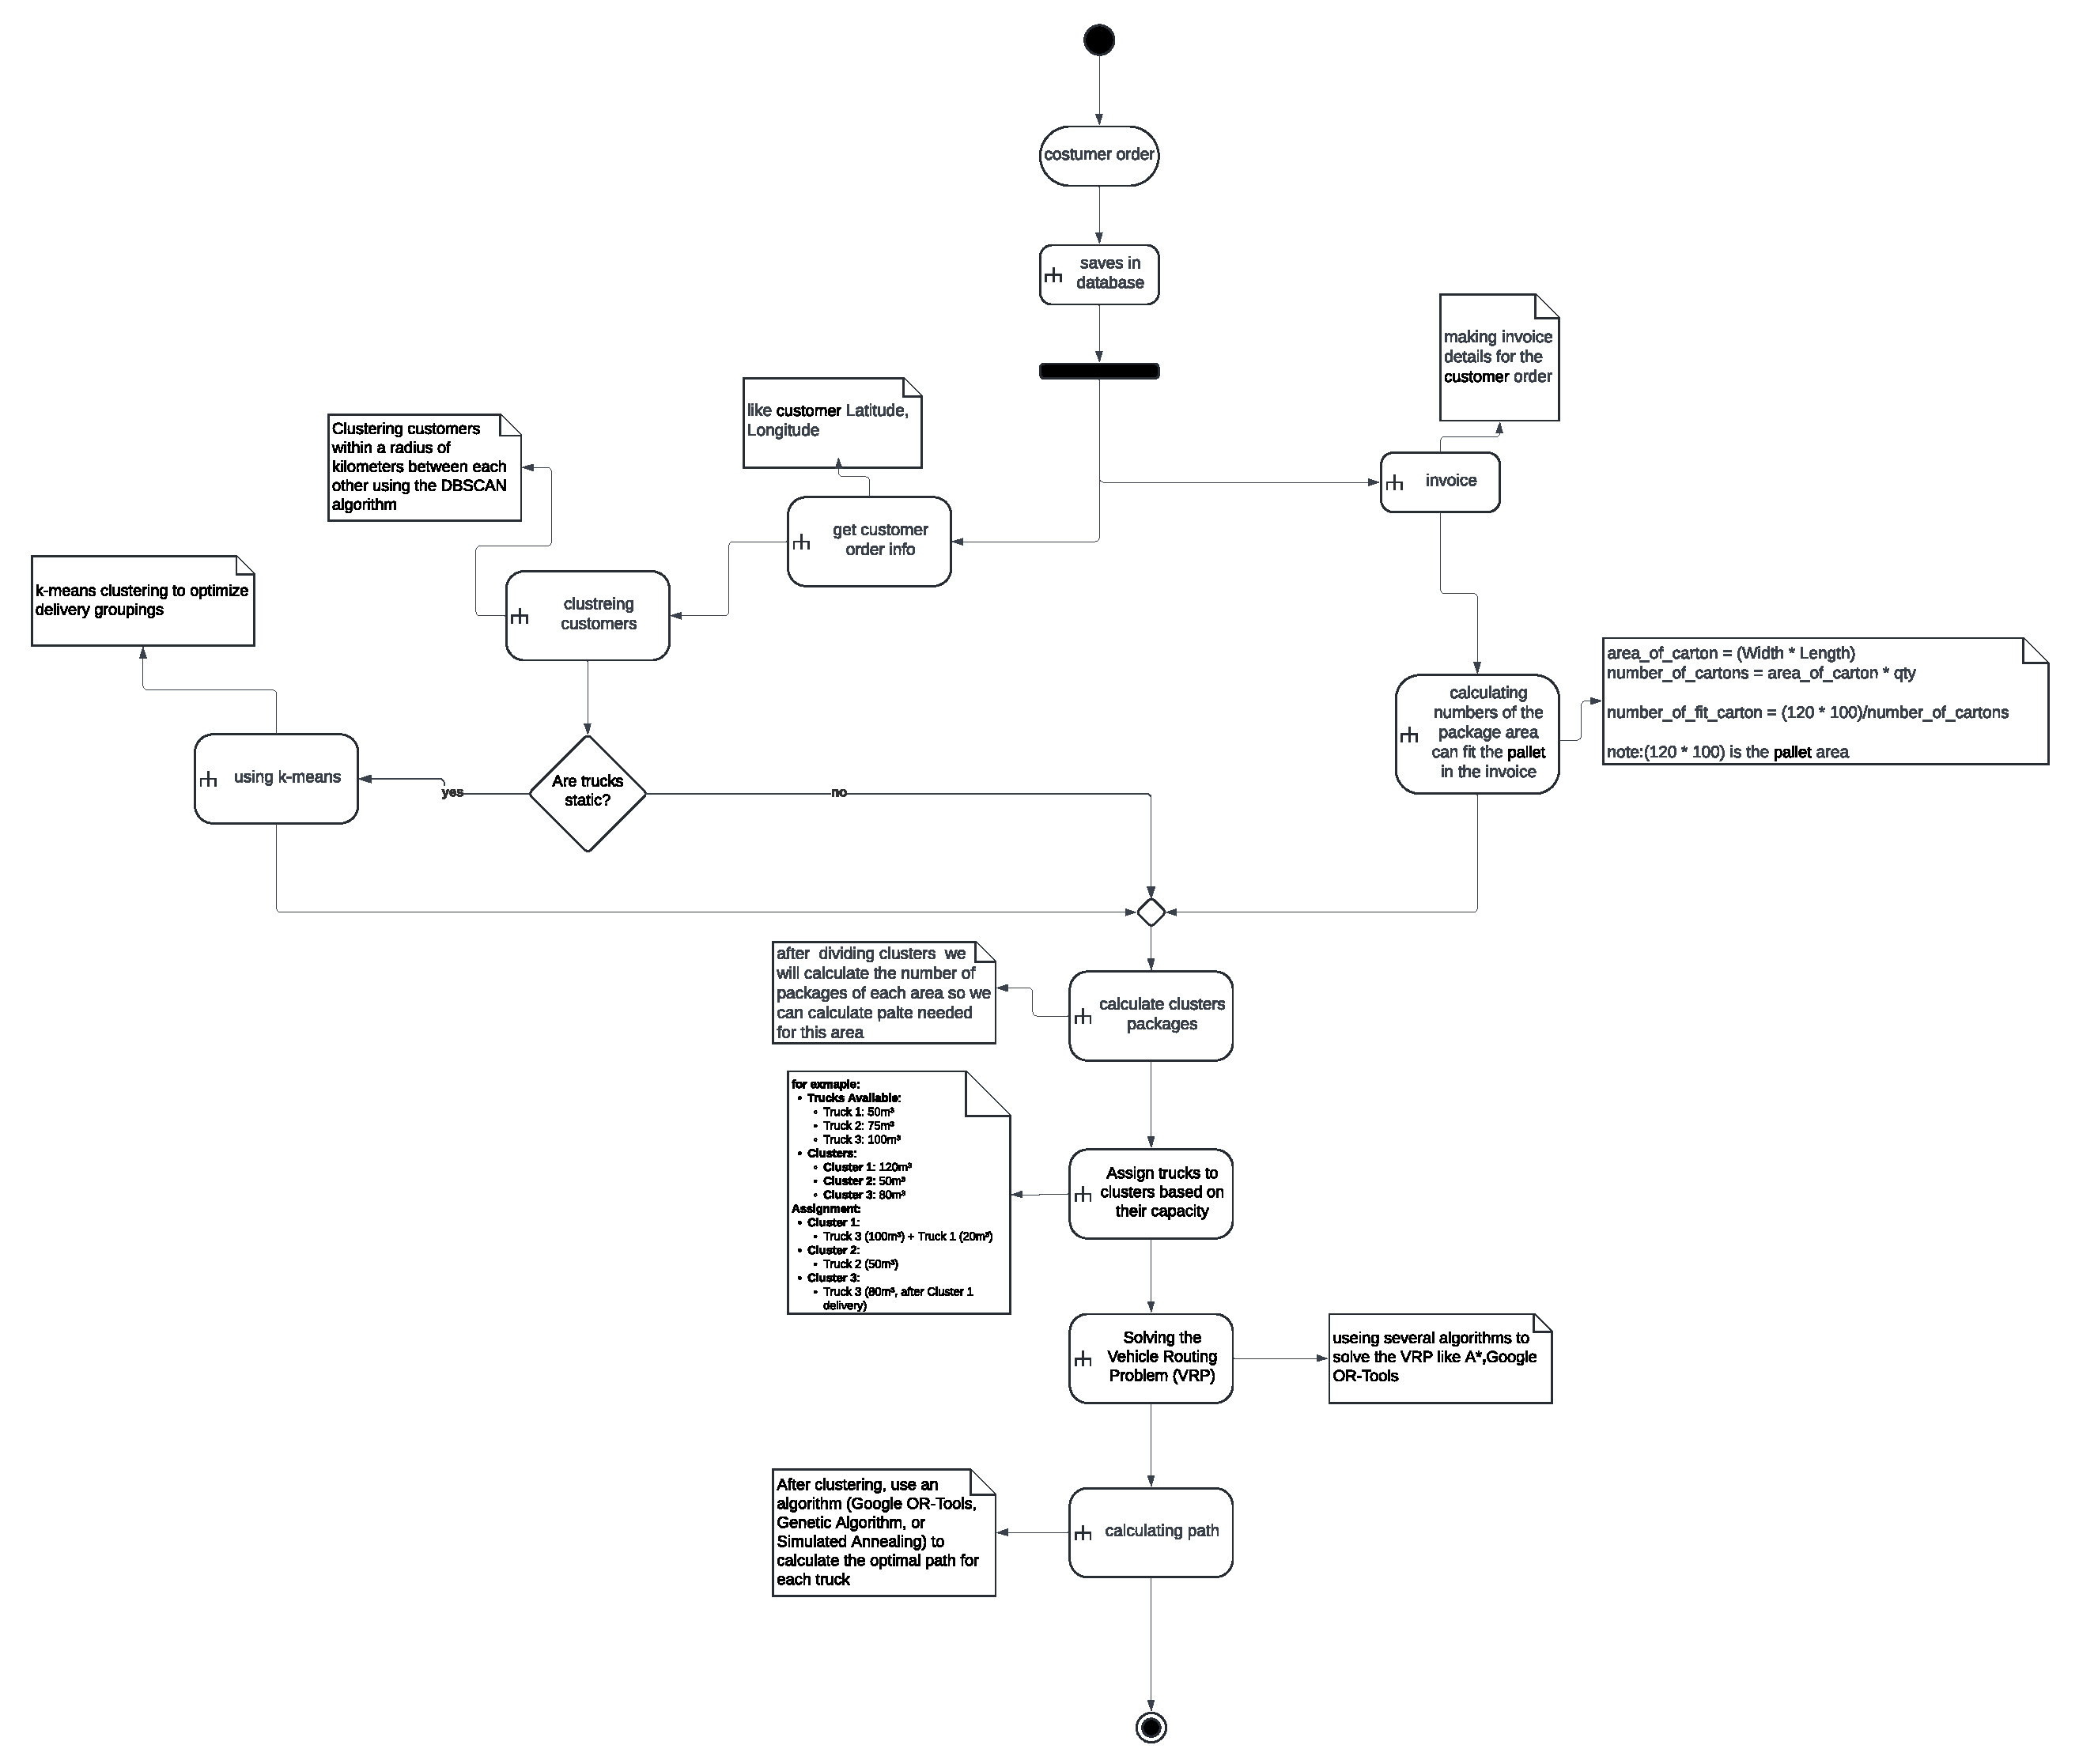
\includegraphics[page=1,width=1.1\textwidth]{TLDR_activity.pdf} 
       % \includegraphics[page=2,width=.45\textwidth]{somemultipagepdf} \\[.5cm]
       % \includegraphics[page=3,width=.45\textwidth]{somemultipagepdf} \\
   \end{tabular}
 \caption{New Database Diagram}
 \label{fig:Test}
\end{figure}






\section{Potential Risks and Mitigation}
There may be resistance to change from staff. To mitigate this, training sessions should be provided
to explain the benefits and how to use the new system.


\section{Conclusion}
Optimizing truck routing will help reduce costs and improve operational efficiency. We encourage
the company to adopt this solution and move forward with further discussions in an upcoming
meeting.





% End Document
\end{document}
